%; whizzy paragraph -pdf xpdf -latex ./whizzypdfptex.sh
%; whizzy-paragraph "^\\\\begin{frame}\\|\\\\emtext"
% latex beamer presentation.
% platex, latex-beamer でコンパイルすることを想定。 

%     Tokyo Debian Meeting resources
%     Copyright (C) 2012 Junichi Uekawa

%     This program is free software; you can redistribute it and/or modify
%     it under the terms of the GNU General Public License as published by
%     the Free Software Foundation; either version 2 of the License, or
%     (at your option) any later version.

%     This program is distributed in the hope that it will be useful,
%     but WITHOUT ANY WARRANTY; without even the implied warreanty of
%     MERCHANTABILITY or FITNESS FOR A PARTICULAR PURPOSE.  See the
%     GNU General Public License for more details.
%     You should have received a copy of the GNU General Public License
%     along with this program; if not, write to the Free Software
%     Foundation, Inc., 51 Franklin St, Fifth Floor, Boston, MA  02110-1301 USA

\documentclass[cjk,dvipdfmx,12pt]{beamer}
\usetheme{Tokyo}
\usepackage{monthlypresentation}

%  preview (shell-command (concat "evince " (replace-regexp-in-string "tex$" "pdf"(buffer-file-name)) "&")) 
%  presentation (shell-command (concat "xpdf -fullscreen " (replace-regexp-in-string "tex$" "pdf"(buffer-file-name)) "&"))
%  presentation (shell-command (concat "evince " (replace-regexp-in-string "tex$" "pdf"(buffer-file-name)) "&"))

%http://www.naney.org/diki/dk/hyperref.html
%日本語EUC系環境の時
\AtBeginDvi{\special{pdf:tounicode EUC-UCS2}}
%シフトJIS系環境の時
%\AtBeginDvi{\special{pdf:tounicode 90ms-RKSJ-UCS2}}

\newenvironment{commandlinesmall}%
{\VerbatimEnvironment
  \begin{Sbox}\begin{minipage}{1.0\hsize}\begin{fontsize}{8}{8} \begin{BVerbatim}}%
{\end{BVerbatim}\end{fontsize}\end{minipage}\end{Sbox}
  \setlength{\fboxsep}{8pt}
% start on a new paragraph

\vspace{6pt}% skip before
\fcolorbox{dancerdarkblue}{dancerlightblue}{\TheSbox}

\vspace{6pt}% skip after
}
%end of commandlinesmall

\title{go / debian での機械学習環境構築について}
\author{齋藤 雄介  ysaito@golangcoder.club}
\date{2018年3月24日}
\logo{
\includegraphics[width=8cm]{image200607/openlogo-light.eps}}

\begin{document}

\begin{frame}
\titlepage{}
\end{frame}

\begin{frame}{参考にした資料}
  Machine Learning with Go (packt publishing)
  %%BoundingBox: 0.00 0.00 362.83 272.13
  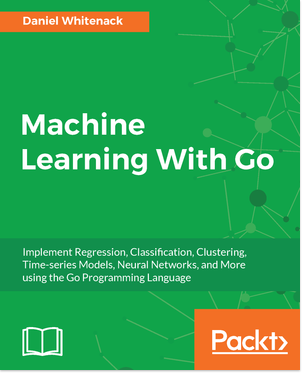
\includegraphics[width=0.8\hsize]{image201803/Shiryo001.png}
\end{frame}


\section{}
%\emtext{}

\begin{frame}[containsverbatim]{伝えたいこと}
機械学習というと python や R が選択肢にあがるが,
Go による機械学習環境構築もメリットがありそう
\begin{itemize}
 \item 静的型安全
 \item 並列計算
 \item ポータビリティや, システムプログラミングとの親和性
\end{itemize}

\end{frame}

\begin{frame}{構築する環境概要}

%%BoundingBox: 0.00 0.00 362.83 272.13
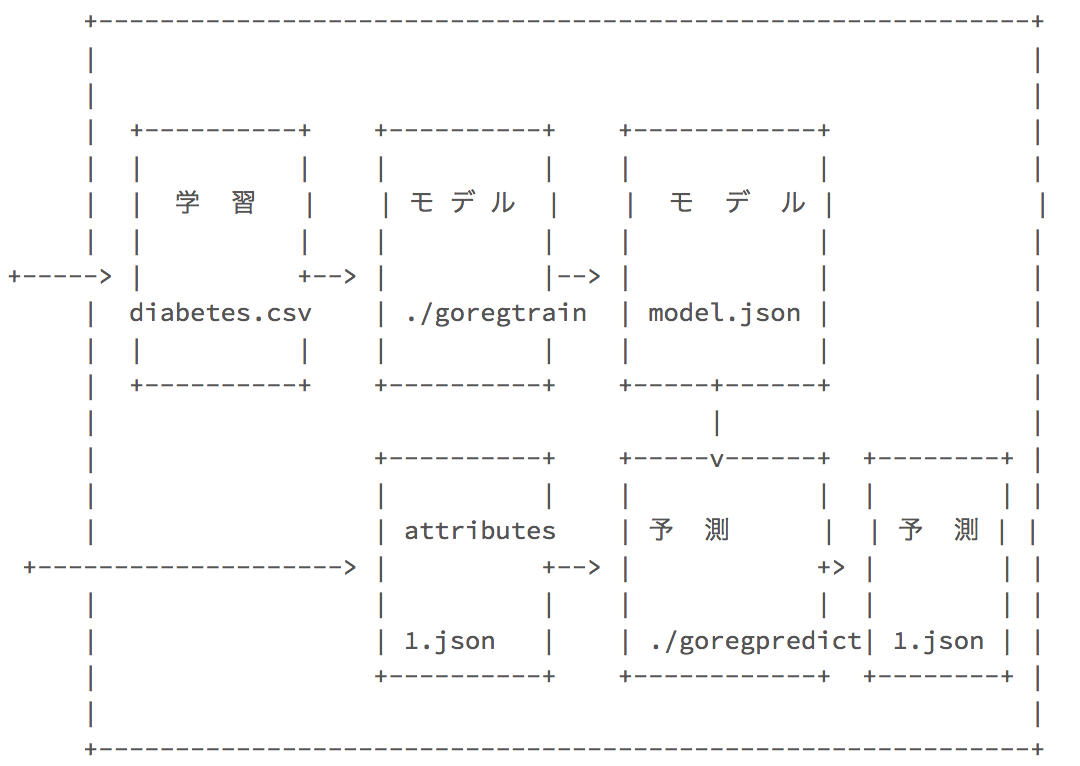
\includegraphics[width=0.8\hsize]{image201803/Shiryo002.png}

\end{frame}

\begin{frame}{debian で構築する動機}

rasbian で構築できれば,
raspberry pi をつなげて, クラスタが作りやすいのでは!

\end{frame}

\begin{frame}{導入するツール}

\begin{itemize}
 \item kubernetes : コンテナオーケストレーションツール (今回は minikube)
 \item docker    : コンテナツール
 \item pachyderm : データバージョニング, データパイプラインツール
\end{itemize}

\end{frame}

\end{document}

;;; Local Variables: ***
;;; outline-regexp: "\\([ 	]*\\\\\\(documentstyle\\|documentclass\\|emtext\\|section\\|begin{frame}\\)\\*?[ 	]*[[{]\\|[]+\\)" ***
;;; End: ***
